\documentclass{article}

\usepackage{amsmath} % math stuff
\usepackage{amssymb} % math stuff
\usepackage{array} % equations and stuff
\usepackage{bm} % bold math
%\usepackage{caption} % suppressed table numbering; incompatible with revtex, and longtable, I think
\usepackage{comment} % comment environment
%\usepackage{enumitem} % customization of enumeration, itemize, and description
\usepackage[T1]{fontenc} % font encoding for special characters, must also use scalable font package
\usepackage[margin=0.8in]{geometry} % paper sizes and margins (but be careful not to mess up pre-defined pages)
\usepackage{graphicx} % for graphics
%\usepackage{helvet} % default font is the helvetica postscript font
\usepackage{lipsum} % lorem ipsum filler text
\usepackage{lmodern} % scalable font?
\usepackage{longtable} % multi-page tables
\usepackage{mathrsfs} % math script font
\usepackage{mhchem} % easier chemical formula
\usepackage{microtype} % allows disabling of ligatures
%\usepackage{newcent} % new century schoolbook font
\usepackage{nicefrac}
\usepackage{parskip} % removes paragraph indentation, and adjusts paragraph skip, as well as list items
%\usepackage{setspace} % adjust text spacing and indents
\usepackage{siunitx} % decimal alignment
\usepackage{subfigure} % divided figures
%\usepackage{tabu} % extra table options
\usepackage{textcomp} % symbols
\usepackage{threeparttablex} % better footnotes with longtable
\usepackage{titling} % title placement
\usepackage{ulem} % strikethrough text
%\usepackage{url} % superceded by hyperref
\usepackage{verbatim} % verbatim environment
\usepackage{xcolor} % colors and color boxes
\usepackage{xspace} % commands that don't eat up white space
\usepackage{hyperref} % links and page setup; should always come last

\hypersetup{
	bookmarks=true,
	colorlinks=true,
	citecolor=blue,
	linkcolor=blue,
	urlcolor=blue,
	pdfstartview={XYZ null null 1.0} % default open view is 100%
}

\DisableLigatures[f]{encoding = *, family = * } % disable ff, fi, fl ligatures, without f option, it also disables -- = endash
\renewcommand{\arraystretch}{1.1} % extra vertical space in tables

\begin{document}

\pagestyle{empty} % don't number pages

% custom title
\begin{center}
{\LARGE Express Riddler}

\vspace{0.15in}

{\Large 18 September 2020}
\end{center}


\section*{Riddle:}

Quoc's lab has a microcentrifuge, a piece of equipment that can separate components of a liquid by spinning around very rapidly.
Liquid samples are pipetted into small tubes, which are then placed in one of the microcentrifuge's 12 slots evenly spaced in a circle.

\begin{center}
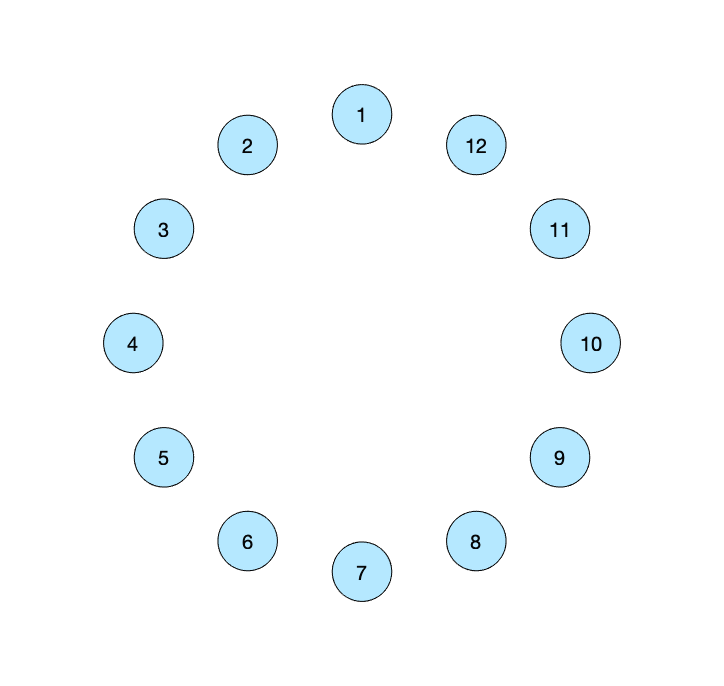
\includegraphics[width=4in]{centrifuge-2.png}
\end{center}

For the microcentrifuge to work properly, each tube must hold the same amount of liquid.
Also, importantly, the center of mass of the samples must be at the very center of the circle — otherwise, the microcentrifuge will not be balanced and may break.

Quoc notices that there is no way to place exactly one tube in the microcentrifuge so that it will be balanced, but he can place two tubes (e.g., in slots 1 and 7).

Now Quoc needs to spin exactly seven samples.
In which slots (numbered 1 through 12, as in the diagram above) should he place them so that the centrifuge will be balanced?

\textit{Extra credit}: Assuming the 12 slots are distinct, how many different balanced arrangements of seven samples are there?

\section*{Solution:}

The most basic way to balance a centrifuge is to distribute a set of $n$ tubes evenly throughout the $N$ slots.
To be able to distribute the tubes, $n$ must divide $N$, and more specifically, assuming $n$ is prime leads to more possible solutions.
In this case, $N=12$, and so $n$ can be 2 or 3.
For $n=2$, the two tubes must be in opposite slots, and there are six ways to do this: 1-7, 2-8, 3-9, 4-10, 5-11, and 6-12.
For $n=3$, the tubes are in every fourth slot, and there are four solutions: 1-5-9, 2-6-10, 3-7-11, and 4-8-12.

These solutions can be combined for larger numbers of tubes.
For example, with four tubes, a solution is 1-2-7-8, which is just two solutions for $n=2$ that don't overlap.
Similarly, a solution with 5 tubes is 2-3-7-8-11, which is a combination $n=2$ and $n=3$ solutions.
One important thing to notice is that if there is a solution for some number $k$ tubes (not necessarily a factor of $N$), then there is also a solution for $N-k$ tubes, which is just the inverse solution.
So in this case, it is actually easier to find solutions for $k=5$ tubes, since each 5-tube solution is a combination of a 2-tube and a 3-tube solution.
Then the solutions for 7 tubes are trivial.

Counting the solutions exhaustively is rather easy.
It is easy to see that for any 2-tube solution, there are exactly two of the four 3-tube solutions which do not overlap.
For example, starting with 1-7, the non-overlapping triplets are 2-6-10 and 4-8-12.
Since there are six 2-tube solutions to begin with, there are a total of twelve 5-tube solutions, and exactly twelve 7-tube solutions. I list them below:

\vspace{0.1in}
\begin{center}
\begin{tabular}{c}
1-2-3-6-7-9-10\\
1-2-4-5-8-9-10\\
1-2-5-6-7-10-11\\
1-2-5-6-8-9-12\\
1-3-4-7-8-9-12\\
1-4-5-6-9-10-12\\
1-4-5-7-8-11-12\\
2-3-4-7-8-10-11\\
2-3-5-6-9-10-11\\
2-3-6-7-8-11-12\\
3-4-5-8-9-11-12\\
3-4-6-7-10-11-12
\end{tabular}
\end{center}


\end{document}